\documentclass[a4paper,12pt]{article}
\usepackage{amsmath}
\usepackage{amssymb}
\usepackage[polish]{babel}
\usepackage{polski}
\usepackage[utf8]{inputenc}
\usepackage{indentfirst}
\usepackage{geometry}
\usepackage{array}
\usepackage[pdftex]{color,graphicx}
\usepackage{subfigure}
\usepackage{afterpage}
\usepackage{setspace}
\usepackage{color}
\usepackage{wrapfig}
\usepackage{listings}
\usepackage{datetime}
\usepackage{titlesec}
\renewcommand{\onehalfspacing}{\setstretch{1.6}}
\geometry{tmargin=2.5cm,bmargin=2.5cm,lmargin=2.5cm,rmargin=2.5cm}
\setlength{\parindent}{1cm}
\setlength{\parskip}{0mm}
\newenvironment{lista}{
\begin{itemize}
  \setlength{\itemsep}{1pt}
  \setlength{\parskip}{0pt}
  \setlength{\parsep}{0pt}
}{\end{itemize}}
\titleformat{\section}[block]{\Large\bfseries\filcenter}{}{1em}{}
\newcommand{\linia}{\rule{\linewidth}{0.4mm}}
\definecolor{lbcolor}{rgb}{0.95,0.95,0.95}
\lstset{
    backgroundcolor=\color{lbcolor},
    tabsize=4,
  language=C++,
  captionpos=b,
  tabsize=3,
  frame=lines,
  numbers=left,
  numberstyle=\tiny,
  numbersep=5pt,
  breaklines=true,
  showstringspaces=false,
  basicstyle=\footnotesize,
  identifierstyle=\color{magenta},
  keywordstyle=\color[rgb]{0,0,1},
  commentstyle=\color{Darkgreen},
  stringstyle=\color{red}
  }
\begin{document}
\noindent
\begin{tabular}{|c|p{11cm}|c|} \hline 
Grupa Wtorek 9.15 & Michał Jaworek, Marcin Kaciuba & \ddmmyyyydate\today \tabularnewline
\hline 
\end{tabular}


\section*{Algorytm Smitha-Watermana - poszukiwanie optymalnych lokalnych dopasowań sekwencji }


\subsection*{Abstrakt}
Algorytmy dopasowania sekwencji znajduje swoje zastosowanie m. in. w bioinformatyce do poszukiwań dopasowań sekwencji nukleotydów i aminokwasów. Algorytm Smitha-Watermana należy do podgrupy rozwiązań zajmujących jest tzw. dopasowaniem lokalnym. W poniższym dokumencie przedstawiono opis prób zrównoleglenia tego algorytmu z wykorzystaniem technologii CUDA. 

\subsection*{Przedostawienie problemu}

Problem dopasowania sekwencji przyjmuje na wejściu dwa ciągi znaków. W ogólnym przypadku, ciągi te mogą składać się z liter dowolnego alfabetu. W przypadku zastosowań bioinformatyczych zazwyczaj ten alfabet jest relatywnie niewielki (np. czteroznakowy "TGAC"). 

Problem tej klasy można interpretować na dwa sposoby. Istnieją rozwiązania analizujące:
\begin{lista}
 \item dopasowanie globalne
\item dopasowanie lokalne
\end{lista}

W przypadku dopasowania globalnego dwa ciągi porównywane są wzdłuż całej sekwencji. Takie rozwiązanie jest wykorzystywane przy analizie jednodomenowych białek. Algorytmem tego typu jest na przykład algorytm Needlemana-Wunscha. Schemat takiego dopasowania przedstawiono poniżej: 

\begin{figure}[h]
  \vspace{5pt}
  \centering
  \begin{center}
  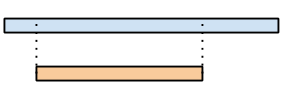
\includegraphics[width=0.5\textwidth]{images/Dopasowanie_globalne.png}
  \end{center}
  \caption{Schemat dopasowania globalnego}
 \end{figure}
  

Lokalny typ dopasowania polega na rozszerzeniu możliwości algorytmów pierwszego typu o zdolność do zauważenia podobieństw w małych obaszarach. Dla przykładu pewne sekwencje mogę być zamienione kolejnością. Ten typ rozwiązania znajduje zastosowanie w analizowaniu białek wielodomenowych.  Poniżej przedstawiono schemat dopasowania tego typu. 

\begin{figure}[h]
  \vspace{5pt}
  \centering
  \begin{center}
  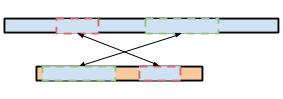
\includegraphics[width=0.5\textwidth]{images/Dopasowanie_lokalne.png}
  \end{center}
  \caption{Schemat dopasowania lokalnego}
 \end{figure}
 
 
Dla uwidocznienia różnicy w działaniu tych dwóch typów algorytmów posłużmy się przykładem następujących ciągów:
\begin{lista}
 \item TGGAACCA
\item ACCATGGA
\end{lista}

Powyższa sekwencja składa się z dwóch czteroliterowych sekwencji umieszczony w różnej kolejności. Poniżej przedstawiono macierze podobieństawa uzyskane przez oba algorytmy wraz ze znalozionymi rozwiązaniami. Proces powstawania macierzy tego typu zostanie opisany w dalszej częście tego dokumentu. 


\begin{figure}[h]
  \vspace{5pt}
  \centering
  \begin{center}
  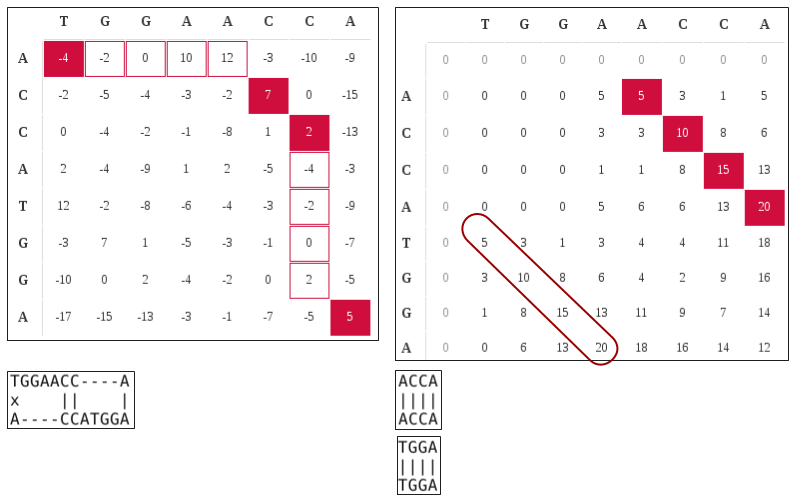
\includegraphics[width=1.0\textwidth]{images/Globalne_lokalne_przyklad.png}
  \end{center}
  \caption{Przykład różnicy w działaniu dopasowania globalnego (po lewo) i dopasowania lokalnego (po prawo)}
 \end{figure}


W przypadku globalnego dopasowania najlepszy uzyskany wynik jest jeden. Algorytm uzaje, że za najpesze dopasowanie należy uznać następującą interpretacje: 
Dla uwidocznienia różnicy w działaniu tych dwóch typów algorytmów posłużmy się przykładem następujących ciągów:
\begin{lista}
 \item Pierwszy znak został podmieniony
\item Natępnie brakuje 4 znaków w drugim ciągu
\item Kolejne dwa znaki pasują do siebie
\item Natępnie brakuje 4 znaków w pierwszym ciągu
\item Ostatnie znaki pasują do siebie
\end{lista}

Jak widać, takie rozwiązanie nie jest w stanie wykryć istoty zadanego przykładu. Dla odmiany dopasowanie lokalne nie narzuca jednego najlepszego rozwiązania. Po zbudowaniu macierzy podobieństwa możemy zauważyć że istnieją dwie ścieżki punktowane w ten sam sposób. Jedna z nich repreztuje informacje o znalezieniu dopasowania podciągów "ACCA", druga o znalezieniu dopasowania podciągów "TGGA". W przypadku dużych ciągów wejściowych powyższe macierze reprezentuje się w odmienny sposób. Przyjmując pewną wartość progową można utworzyć wykres tego typu:

\begin{figure}[h]
  \vspace{5pt}
  \centering
  \begin{center}
  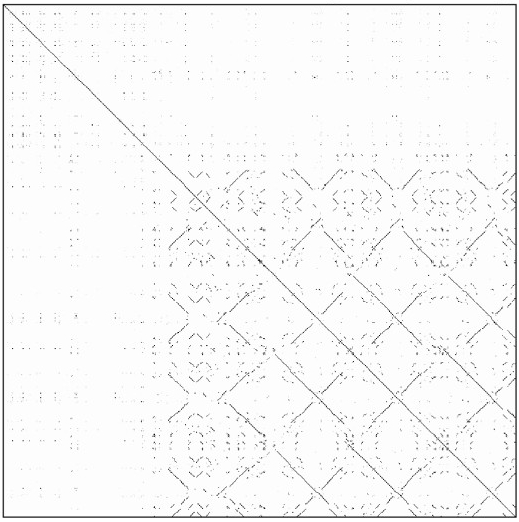
\includegraphics[width=0.6\textwidth]{images/macierz.png}
  \end{center}
  \caption{Przykład wizualnej reprezentacji macierzy podobieństwa dla algorytmu dopasowania lokalnego}
\end{figure}

Dzięki takiemu przedstawieniu wyników możliwe jest zwrócenie uwagi na fragmenty zawierające istotne podobieństwo. 


\subsection*{Algorytm Smitha-Watermana w ujęciu sekwencyjnym}

Algorym Smitha-Watermana należy do klasy algorytmów dynamicznych. Składa się z się z dwóch etapów:
\begin{lista}
 \item Tworzenie macierzy podobieństwa
\item Otwarzanie optymalnej ścieżki (ang. backtracking)
\end{lista}

W pierwszym etapie zostaje utworzona pusta macierz. Jej wiersze odpowiadają kolejnym znakom pierwszego ciągu, kolumny kolejnym znakom drugiego ciągu. Komórki znajdujące się na przecięcie opisują punktacje określającą w jakim stopniu dopasowanie danych dwóch znaków jest poprawne. 

W celu wypełnienia powyższej macierzy należy zauwazyć, że przy porównywaniu dwóch ciągów można mieć miesce trzy sytuacje przedstawione na poższym schemacie.

\begin{figure}[h]
  \vspace{5pt}
  \centering
  \begin{center}
  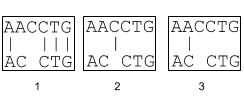
\includegraphics[width=0.6\textwidth]{images/TypySytuacjiPrzyDopasowaniu.png}
  \end{center}
  \caption{Możliwe sytacje w trakcie porównywania ciągów: (1 - dopasowanie, 2 - przerwa, 3 - zamiana)}
 \end{figure}


Dwa ciągi są do siebie podobne gdy mamy więcej sytuacji typu 1 ("dopasowanie") niż sytuacji typów 2 ("przerwa"), 3 ("zamiana"). W związku z tym spostrzeżeniem w trakcie wypełniania macierzy wartościami będziemy dodatnio punktować "dopasowania", podczas gdy "przerwy" i "zamiany" będę punktowane ujemnie. Dokładne wartości punktacji nie są elementem specyfikacji algorytmu i są dobierane w zależności od rozpatrywanego problemu. Daje to możliwość porównywania ciągów w sposób traktujący "przerwy" mniej restrykcyjnie niż "zamiany" (lub odrotnie). 

W celu opisy kroków algorytmy posłużono się przykładem. Schemat przedstawiony na rysunku 6. prezentuje pierwsze kroki wykonywane w celu wypełnienia macierzy podobieństwa. Przedstawiono przypadek dla danych wejściowych: TGGA, TGA oraz dla parametrów:
\begin{lista}
\item Punktacja za dopasowanie: 5
\item Punktacja za zamiane: -3
\item Punktacja za przerwe: -2
\end{lista}

\begin{figure}[h]
  \vspace{5pt}
  \centering
  \begin{center}
  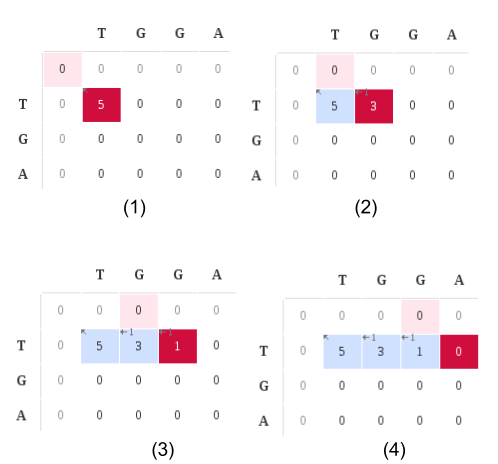
\includegraphics[width=0.6\textwidth]{images/SchematDzialaniaAlgorytmu.png}
  \end{center}
  \caption{Pierwsze cztery kroki wykonaniu algorytmu Smitha-Watermana dla danych wejściowych: TGGA, TGA}
 \end{figure}

Na początku macierz wypełniona jest zerami. Należy zwrócić uwagę na istnienie dodatkowego wiersza i kolumny (oznaczone na schematach szarą czcionką). Komórki rozpatrywane są wiersz po wierszy. Dla każdej komórki wykonywana jest sekwencja kroków mająca odpowiedzieć na następujące pytanie: "Przez którego z sąsiadów należy poprowadzić ścieżkę dopasowania tak, żeby w obecnej komórce osiągnąć najlepszy wyniki?". Przy odpowiedzi na to pytanie rozpatrywane są komórki:
\begin{lista}
\item Na lewo - odpowiadająca wprowadzeniu przerwy w pierwszym ciągu
\item Powyżej - odpowiadająca wprowadzeniu przerwy w drugim ciągu
\item Na skos (powyżej i na lewo) - w zależności od przypadku odpowiadająca wprowadzeniu zamiany lub dopasowania.
\end{lista}

Tą procedurę można przedstawić w pseudokodzie w następujący sposób. 

\begin{lstlisting}
	int fromLeft = valueOfCellOnLeft - penaltyForGap;
	int fromUp = valueOfCellOnUp - penaltyForGap;
	int fromDiagonal;
	if(letterInRow == letterInCol){
		fromDiagonal = valueOfCellInDiagonal + bonusOfMatch;
	}else{
		fromDiagonal = valueOfCellInDiagonal + penaltyForReplacement;
	}
	int	valueOfThisCell = max(fromLeft, fromUp, fromDiagonal);
	rememberDecision();
\end{lstlisting}

Prześledźmy kolejne kroki wykonania przykładu z rysunku 6. Warto przy tej okazji zwrócić uwagę na fakt, że w algorytmie Smitha-Watermana celowo unika się wprowadzania do macierzy ujemnych wartości. Względu na to w poniższym opisie zastosowano znak $\simeq$ wszędzie tam, gdzie zamiast wartości ujemnej podstawiane jest 0.

W kroku 1:
\begin{lista}
\item Wybranie drogi z lewej strony dawałoby: 0 + (-2) $\simeq$ 0
\item Wybranie drogi z góry dawałoby : 0 + (-2) $\simeq$ 0
\item Ze względu na to, że litery w kolumnach (T) i rzędach (T) są takie same przejście na skos dawałoby: 0 + 5 = 5
\item Najbardziej opłacalnym ruchem jest przejście na skos więc zapamiętujemy ten ruch i nadajemy komórce wartość 5
\end{lista}

W kroku 2:
\begin{lista}
\item Wybranie drogi z lewej strony dawałoby: 5 + (-2) = 3
\item Wybranie drogi z góry dawałoby : 0 + (-2) $\simeq$ 0
\item Ze względu na to, że litery w kolumnach (G) i rzędach (T) niesą takie same na skos dawałoby: 0 + (-3) $\simeq$ 0
\item Najbardziej opłacalnym ruchem jest przejście z lewej strony więc zapamiętujemy ten ruch i nadajemy komórce wartość 3
\end{lista}
W kroku 3:
\begin{lista}
\item Wybranie drogi z lewej strony dawałoby: 3 + (-2) = 1
\item Wybranie drogi z góry dawałoby : 0 + (-2) $\simeq$ 0
\item Ze względu na to, że litery w kolumnach (G) i rzędach (T) niesą takie same na skos dawałoby: 0 + (-3) $\simeq$ 0
\item Najbardziej opłacalnym ruchem jest przejście z lewej strony więc zapamiętujemy ten ruch i nadajemy komórce wartość 1
\end{lista}
W kroku 4:
\begin{lista}
\item Wybranie drogi z lewej strony dawałoby: 1 + (-2) $\simeq$ 0
\item Wybranie drogi z góry dawałoby : 0 + (-2) $\simeq$ 0
\item Ze względu na to, że litery w kolumnach (A) i rzędach (T) niesą takie same na skos dawałoby: 0 + (-3) $\simeq$ 0
\item W tym momencie wszystkie drogi dają taką samą wartośc nie zapamiętujemy kierunku i nadajemy komórce wartość 0.
\end{lista}


Po wykonaniu analogicznych kroków dla wszystkich komórek macierzy otrzymamy następujący stan:
\begin{figure}[h]
  \vspace{5pt}
  \centering
  \begin{center}
  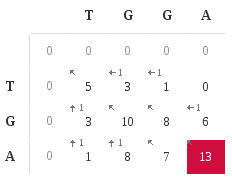
\includegraphics[width=0.5\textwidth]{images/SchematDzialaniaAlgorytmuPelnaMacierz.png}
  \end{center}
  \caption{Całkowicie wypełniona macierz dopasowania algorytmu Smitha-Watermana dla danych wejściowych: TGGA, TGA}
 \end{figure}


W tym momencie macierz jest gotowa do wykonania drugiej fazy - backtrackingu. Polega ona na znalezieniu maksymalnej komórki i zapisaniu wszystkich kroków, które doprowadziły to ustalenie jej wartości. Poniżej przedstawiono macierz z nasiesioną ścieżką metodą backtrackingu. 

Po wykonaniu analogicznych kroków dla wszystkich komórek macierzy otrzymamy stan przedstawiony na rysunku 8.
\begin{figure}[h]
  \vspace{5pt}
  \centering
  \begin{center}
  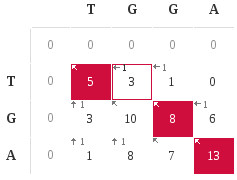
\includegraphics[width=0.5\textwidth]{images/SchematDzialaniaAlgorytmuPelnaMacierzBacktracking.png}
  \end{center}
  \caption{Backtracking dla algorytmu Smitha-Watermana dla danych wejściowych: TGGA, TGA}
 \end{figure}

W efekcie uzyskany wyniki to: [$\nwarrow, \leftarrow, \nwarrow, , \nwarrow$] co należy odczytać jako: [dopasowanie, przerwa, dopasowanie, dopasowanie]. 
Odpowiada do dopasowaniu przedstawionym na rysunku 9. 
\begin{figure}[h]
  \vspace{5pt}
  \centering
  \begin{center}
  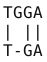
\includegraphics[width=0.1\textwidth]{images/uzyskaneDopasowanie.png}
  \end{center}
  \caption{Wynika dziłania algorytmu Smitha-Watermana dla danych wejściowych: TGGA, TGA}
 \end{figure}

\subsection*{Zarys technologii CUDA}
W ostatnich czasach zwiększanie wyników CPU przez zwiększanie częstotliwości zegara jednak przestało to być skutenczne. Zaczęto iść w stronę zwiększanie liczby rdzeni. Co aktualnie w przypadku procesorów jest kontynuowane. Mimio tych starań okazuję się ze karty graficzne są szybsze.
	Atualnie karty graficzne posiadają setki rdzeni i bardzo szybką pamięć co pozwala przy odpowiednio napisanym algorytmie uzyksanie bardzo dużego przyspieszenia. Widać to na przykład w przypadku łamania haseł, dzięki obliczeniom na karcie graficzne czas metody bruteforce bardzo się skraca. 
\begin{figure}[h]
  \vspace{5pt}
  \centering
  \begin{center}
  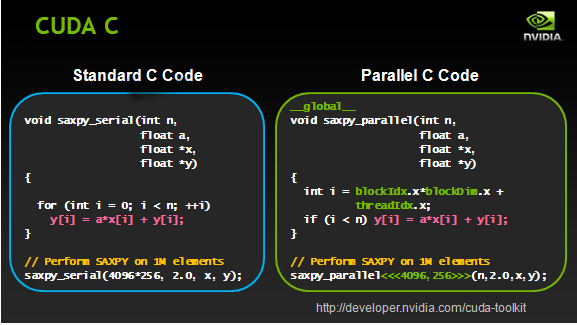
\includegraphics[width=0.4\textwidth]{images/cuda.png}
  \end{center}
  \caption{Porównanie progamu sekewncyjnego z równoległy }
 \end{figure}
 Przyspieszenie to nie jest tak łatwe do uzyskania jak przykładowo w OpenMP gdzie stosuje się dyrektywy. Aby uzyskać znaczne przyszpiesznie na kartach graficznych należy odpowiednio przygotować algortym. W przypadku uruchamiania go na GPU kod kernela(pojedynczej funkcji) wykonywany jest przez setki wątków. Ważne jest też używanie szybkiej pamięci karty.

\subsection*{Model zwrónoleglenia Algorytmu Smitha-Watermana}
Lorem ipsum dolor sit amet, consectetur adipiscing elit. Cras sed velit nec nibh varius suscipit. Curabitur nisi purus, porttitor in urna ut, tincidunt aliquam leo. Integer sit amet nisi egestas, congue tellus nec, gravida tellus. Nulla facilisi. Quisque ultrices sem sed arcu mattis, in eleifend lectus imperdiet. Donec ullamcorper cursus tortor, in interdum sem imperdiet non. Aliquam sit amet viverra nisl, vitae ullamcorper dolor. Pellentesque varius ex a urna blandit, ac volutpat sapien feugiat. Pellentesque habitant morbi tristique senectus et netus et malesuada fames ac turpis egestas. Nulla posuere ligula ligula, ut ullamcorper nulla tempor vitae.

Vestibulum faucibus ex dolor, non suscipit enim sagittis eget. Cras et condimentum elit. Integer porta, quam ac posuere efficitur, magna mauris finibus nisi, at egestas augue diam sed risus. Ut nec nisi quis nunc sagittis volutpat at viverra eros. Donec ut porttitor orci. Mauris eget eleifend neque, id condimentum tortor. Nunc lobortis quam mi, aliquet varius dolor tempus non. Lorem ipsum dolor sit amet, consectetur adipiscing elit.

Class aptent taciti sociosqu ad litora torquent per conubia nostra, per inceptos himenaeos. Nam sed auctor ex. Praesent tempus ipsum sit amet eros tempus, id ornare nulla vulputate. Nullam lobortis mi leo, ac tincidunt est volutpat dapibus. Pellentesque faucibus maximus suscipit. Duis vitae turpis in nisi condimentum finibus quis a arcu. Donec magna massa, elementum rutrum ligula at, dignissim blandit sem. Vivamus est nisl, aliquam ac tellus ac, egestas consectetur erat. Morbi commodo dui non ipsum vehicula dapibus.
\subsection*{Wnioski}
Lorem ipsum dolor sit amet, consectetur adipiscing elit. Cras sed velit nec nibh varius suscipit. Curabitur nisi purus, porttitor in urna ut, tincidunt aliquam leo. Integer sit amet nisi egestas, congue tellus nec, gravida tellus. Nulla facilisi. Quisque ultrices sem sed arcu mattis, in eleifend lectus imperdiet. Donec ullamcorper cursus tortor, in interdum sem imperdiet non. Aliquam sit amet viverra nisl, vitae ullamcorper dolor. Pellentesque varius ex a urna blandit, ac volutpat sapien feugiat. Pellentesque habitant morbi tristique senectus et netus et malesuada fames ac turpis egestas. Nulla posuere ligula ligula, ut ullamcorper nulla tempor vitae.

Vestibulum faucibus ex dolor, non suscipit enim sagittis eget. Cras et condimentum elit. Integer porta, quam ac posuere efficitur, magna mauris finibus nisi, at egestas augue diam sed risus. Ut nec nisi quis nunc sagittis volutpat at viverra eros. Donec ut porttitor orci. Mauris eget eleifend neque, id condimentum tortor. Nunc lobortis quam mi, aliquet varius dolor tempus non. Lorem ipsum dolor sit amet, consectetur adipiscing elit.

Class aptent taciti sociosqu ad litora torquent per conubia nostra, per inceptos himenaeos. Nam sed auctor ex. Praesent tempus ipsum sit amet eros tempus, id ornare nulla vulputate. Nullam lobortis mi leo, ac tincidunt est volutpat dapibus. Pellentesque faucibus maximus suscipit. Duis vitae turpis in nisi condimentum finibus quis a arcu. Donec magna massa, elementum rutrum ligula at, dignissim blandit sem. Vivamus est nisl, aliquam ac tellus ac, egestas consectetur erat. Morbi commodo dui non ipsum vehicula dapibus.

\subsection*{Źródła}
Łukasz Ligowski, Witold Rudnicki - AN EFFICIENT IMPLEMENTATION OF SMITH WATERMAN ALGORITHM ON GPU USING CUDA, FOR MASSIVELY PARALLEL SCANNING OF SEQUENCE DATABASES

E. Banachowicz Bioinformatyka - wykład monograficzny 
http://opal.przyjaznycms.pl/



\end{document}
